\documentclass[12pt,twoside,onecolumn]{article}
\usepackage{a4}
\usepackage[margin=0.95in]{geometry}
\usepackage[utf8]{inputenc}
\usepackage[T1]{fontenc}
\usepackage{hyperref}
\usepackage{url}
\usepackage{tikz}
\usepackage[multiple]{footmisc}
\begin{document}

\section*{S\o knad om utsettelse av masteroppgaven}
Vi s\o ker herved en utsettelse grunnet tekniske problemmer med programvare. 
If\o lge \textbf{4.3.5 Regler for deltidsstudium, permisjon, utsatt levering av masteroppgave, og forsinkelse i studiet}
kan det \emph{innvilges utsatt innlevering av masteroppgaven ved uforskyldte problemer med prosjektet}.

I forbindelse med sin masteroppgave utvikler studenten programvare som avhenger av Python bibloteket SymPy.
Studenten benytter et biblotek som er under utvikling\footnote{\url{http://docs.sympy.org/dev/modules/diffgeom.html}}, 
og har m\aa tte bruke en god del av sin tid på feils\o king. Hvor det ofte har vist seg at feilen skyldes problemmer med 
Python bibloteket SymPy. Stundenten har s\o kt 
hjelp\footnote{\url{http://stackoverflow.com/search?q=user:3352179+[sympy]}}\footnote{\url{https://groups.google.com/forum/\# !forum/sympy}}
fra (blant annet) utvikelere av Sympy bibloteket. Dette i seg selv er problematisk siden SymPy.diffgeom bibloteket 
blir vedlikeholdt og videreutviklet av veldig f{\aa} mennesker.
\\

Vi s\o ker dermed en utsettelse p{\aa} to uker til mandag den 30. november.
\\
\\

\vspace{60mm}
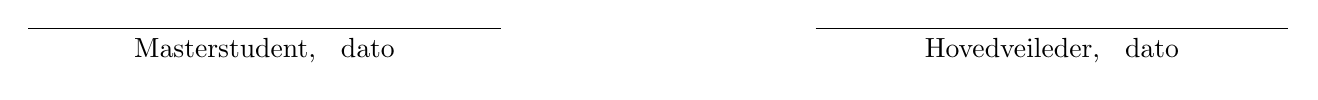
\begin{tikzpicture}
\draw (0,0) -- (6,0) node[below]{\hspace{-60mm}Masterstudent, \hspace{2mm}dato};
\draw (10,0) -- (16,0)node[below]{\hspace{-60mm}Hovedveileder, \hspace{2mm}dato};
\end{tikzpicture}

\end{document}